\section{Qsim::VmQInst Struct Reference}
\label{structQsim_1_1VmQInst}\index{Qsim::VmQInst@{Qsim::VmQInst}}
{\tt \#include $<$qsim.h$>$}

Inheritance diagram for Qsim::VmQInst:\nopagebreak
\begin{figure}[H]
\begin{center}
\leavevmode
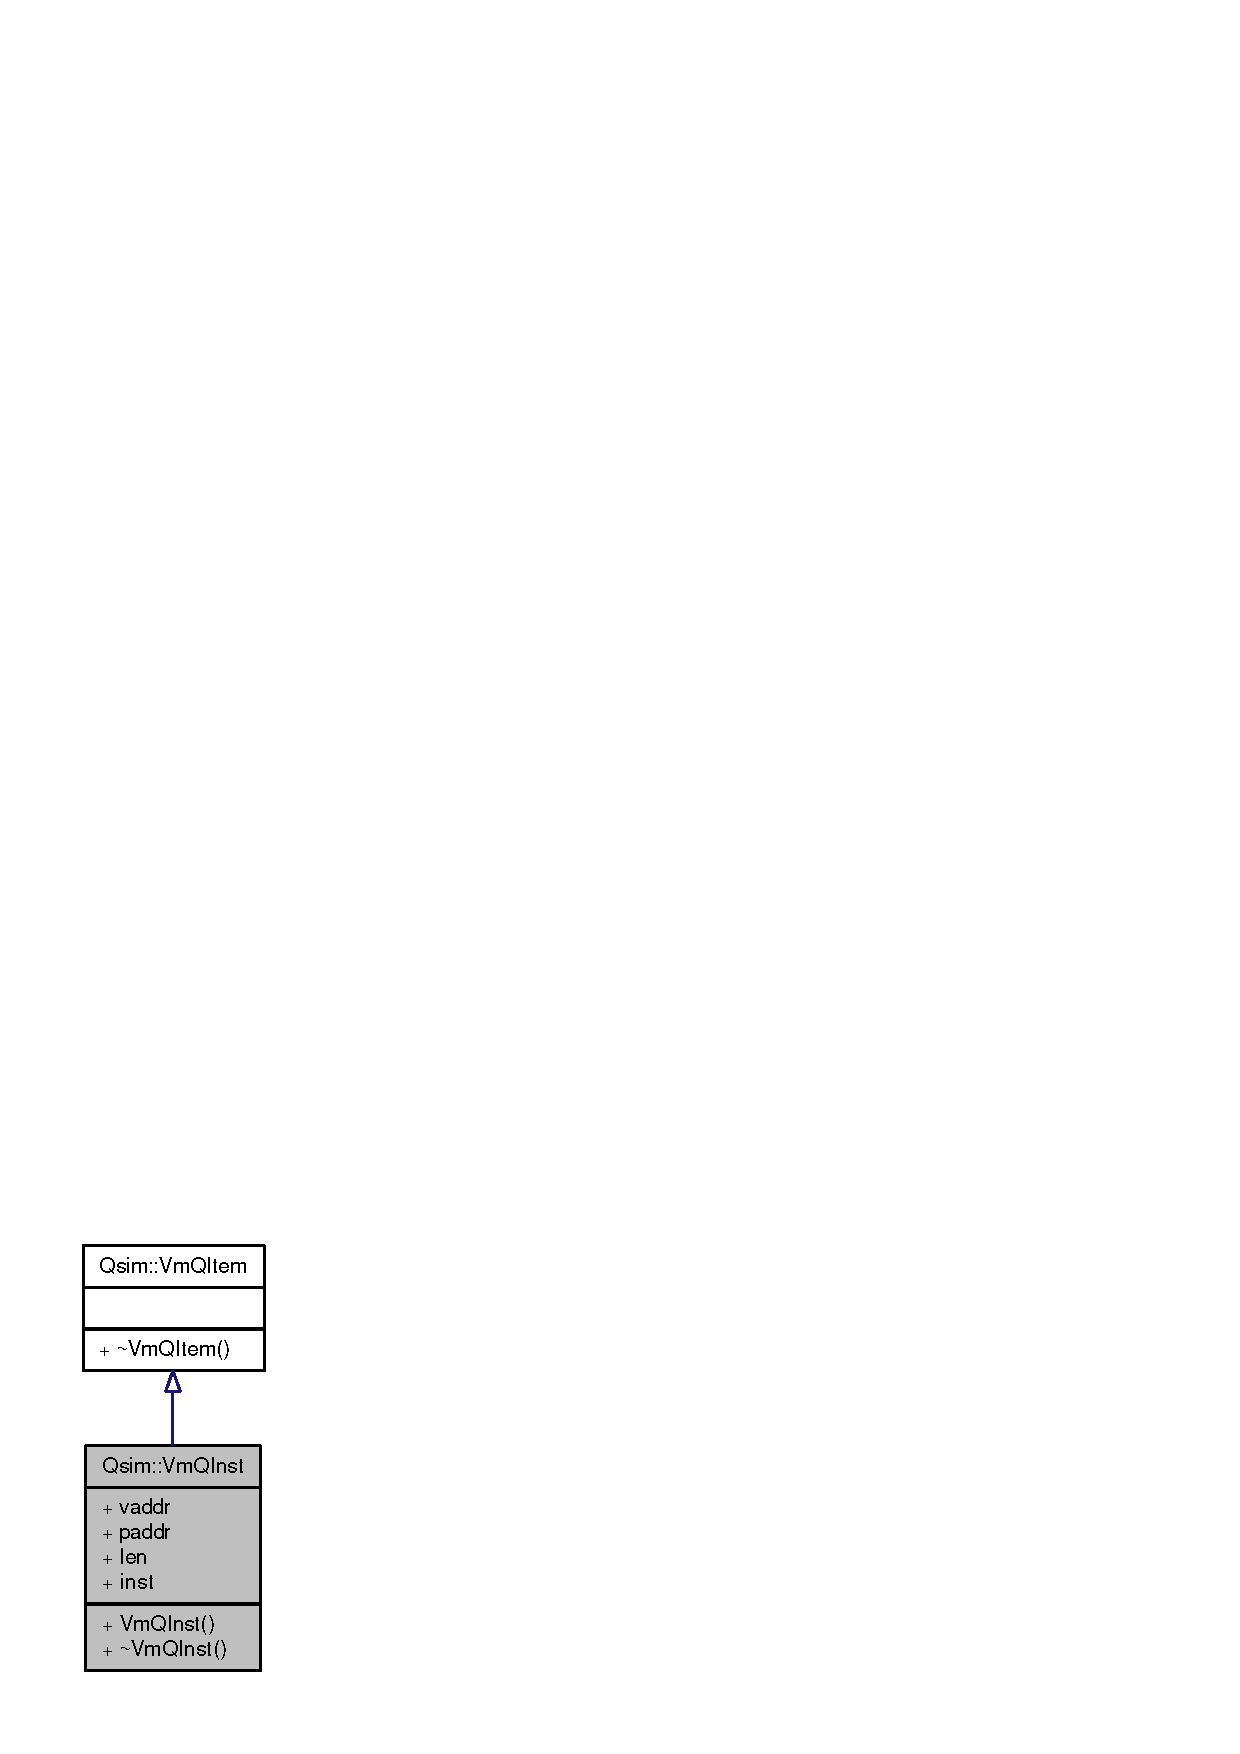
\includegraphics[width=130pt]{structQsim_1_1VmQInst__inherit__graph}
\end{center}
\end{figure}
Collaboration diagram for Qsim::VmQInst:\nopagebreak
\begin{figure}[H]
\begin{center}
\leavevmode
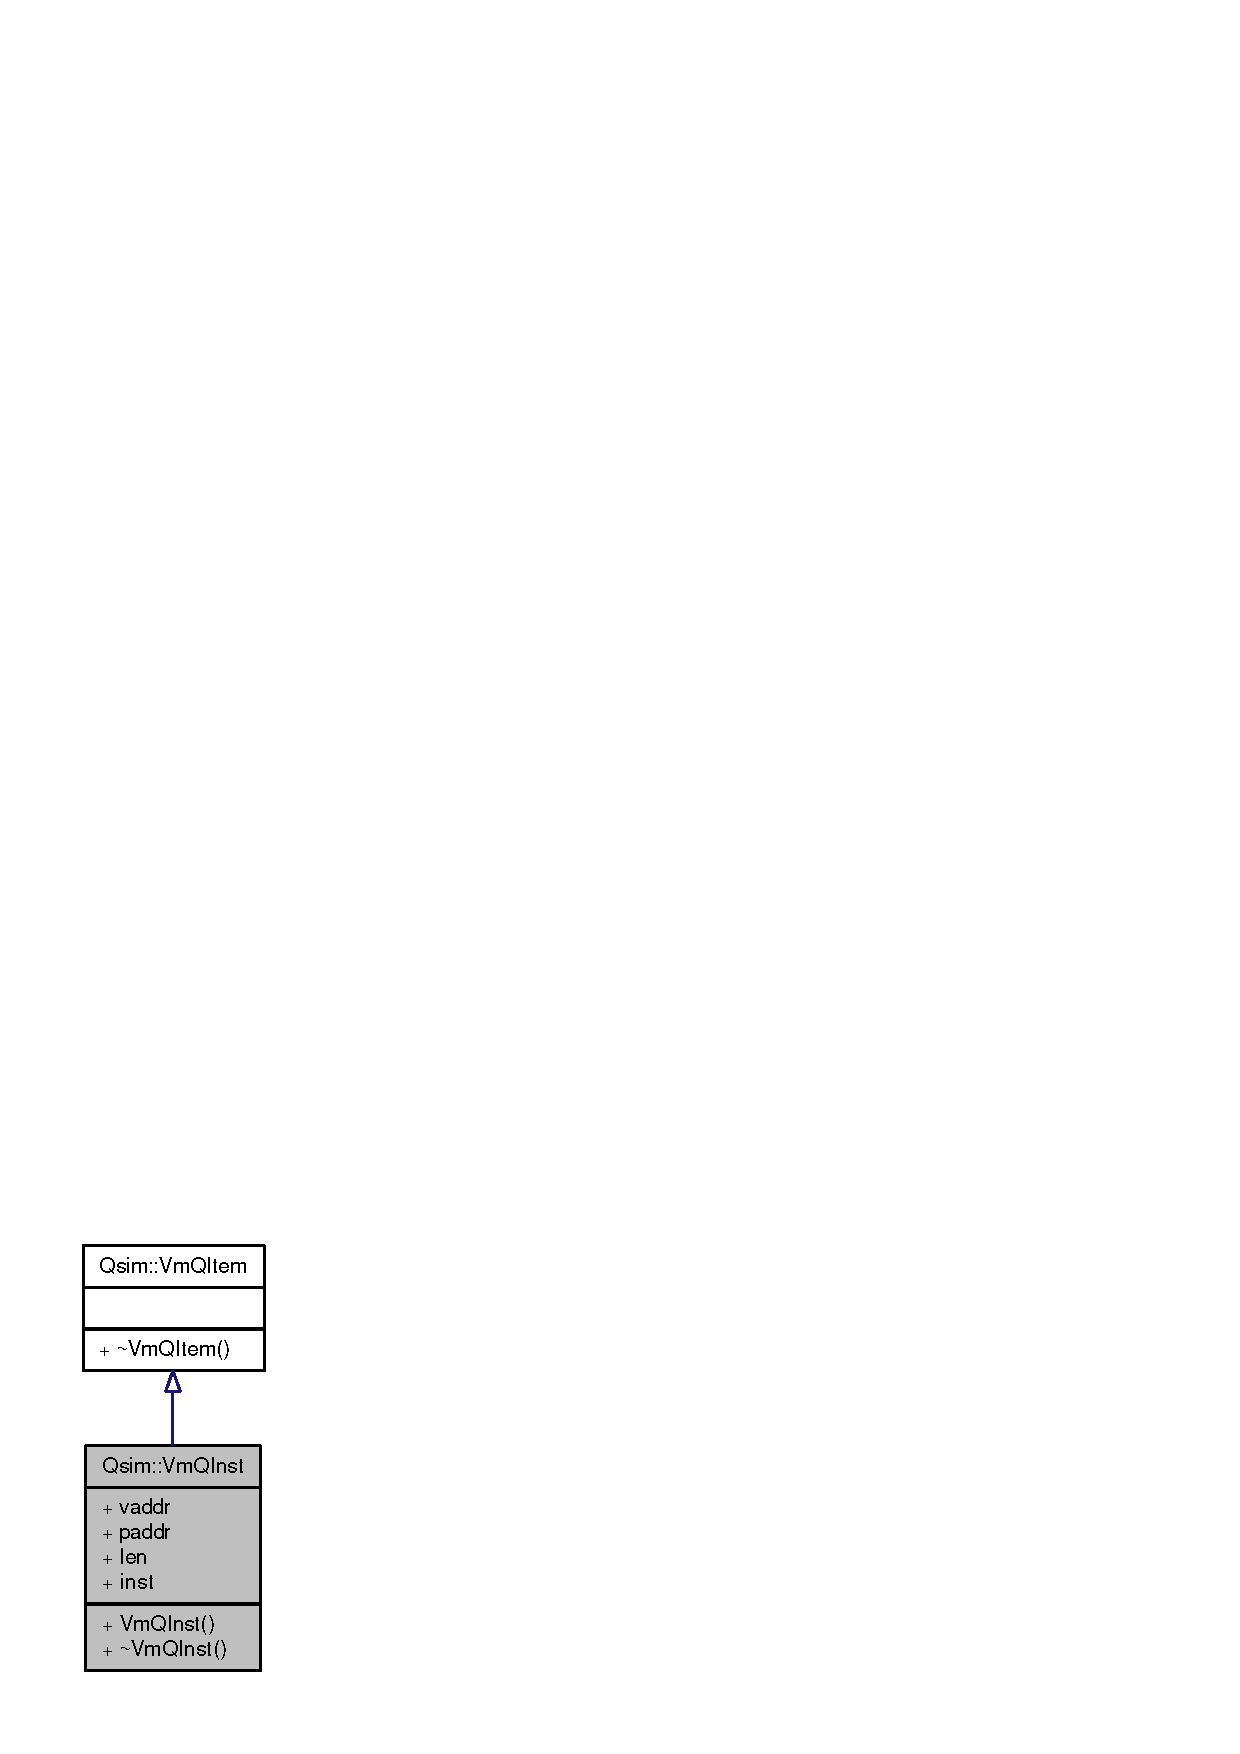
\includegraphics[width=130pt]{structQsim_1_1VmQInst__coll__graph}
\end{center}
\end{figure}
\subsection*{Public Member Functions}
\begin{CompactItemize}
\item 
{\bf VmQInst} (uint64\_\-t {\bf vaddr}, uint64\_\-t {\bf paddr}, uint8\_\-t {\bf len}, uint8\_\-t {\bf data}[$\,$])
\item 
{\bf $\sim$VmQInst} ()
\end{CompactItemize}
\subsection*{Public Attributes}
\begin{CompactItemize}
\item 
uint64\_\-t {\bf vaddr}
\item 
uint64\_\-t {\bf paddr}
\item 
uint8\_\-t {\bf len}
\item 
uint8\_\-t $\ast$ {\bf inst}
\end{CompactItemize}


\subsection{Detailed Description}


Definition at line 92 of file qsim.h.

\subsection{Constructor \& Destructor Documentation}
\index{Qsim::VmQInst@{Qsim::VmQInst}!VmQInst@{VmQInst}}
\index{VmQInst@{VmQInst}!Qsim::VmQInst@{Qsim::VmQInst}}
\subsubsection[{VmQInst}]{\setlength{\rightskip}{0pt plus 5cm}Qsim::VmQInst::VmQInst (uint64\_\-t {\em vaddr}, \/  uint64\_\-t {\em paddr}, \/  uint8\_\-t {\em len}, \/  uint8\_\-t {\em data}[$\,$])\hspace{0.3cm}{\tt  [inline]}}\label{structQsim_1_1VmQInst_407b4fab9bf291628eb86f22608330b1}




Definition at line 93 of file qsim.h.

References inst.\index{Qsim::VmQInst@{Qsim::VmQInst}!$\sim$VmQInst@{$\sim$VmQInst}}
\index{$\sim$VmQInst@{$\sim$VmQInst}!Qsim::VmQInst@{Qsim::VmQInst}}
\subsubsection[{$\sim$VmQInst}]{\setlength{\rightskip}{0pt plus 5cm}Qsim::VmQInst::$\sim$VmQInst ()\hspace{0.3cm}{\tt  [inline]}}\label{structQsim_1_1VmQInst_4e681e9d722fde229a5d604df7d8a8f0}




Definition at line 99 of file qsim.h.

References inst.

\subsection{Member Data Documentation}
\index{Qsim::VmQInst@{Qsim::VmQInst}!inst@{inst}}
\index{inst@{inst}!Qsim::VmQInst@{Qsim::VmQInst}}
\subsubsection[{inst}]{\setlength{\rightskip}{0pt plus 5cm}uint8\_\-t$\ast$ {\bf Qsim::VmQInst::inst}}\label{structQsim_1_1VmQInst_e184916566a7a97022e53176bd4e55bd}




Definition at line 103 of file qsim.h.

Referenced by VmQInst(), and $\sim$VmQInst().\index{Qsim::VmQInst@{Qsim::VmQInst}!len@{len}}
\index{len@{len}!Qsim::VmQInst@{Qsim::VmQInst}}
\subsubsection[{len}]{\setlength{\rightskip}{0pt plus 5cm}uint8\_\-t {\bf Qsim::VmQInst::len}}\label{structQsim_1_1VmQInst_7b14b6c249d425da92725a8f850d6c92}




Definition at line 102 of file qsim.h.\index{Qsim::VmQInst@{Qsim::VmQInst}!paddr@{paddr}}
\index{paddr@{paddr}!Qsim::VmQInst@{Qsim::VmQInst}}
\subsubsection[{paddr}]{\setlength{\rightskip}{0pt plus 5cm}uint64\_\-t {\bf Qsim::VmQInst::paddr}}\label{structQsim_1_1VmQInst_f5c063db3a58690ef5d54166a4c6468f}




Definition at line 101 of file qsim.h.\index{Qsim::VmQInst@{Qsim::VmQInst}!vaddr@{vaddr}}
\index{vaddr@{vaddr}!Qsim::VmQInst@{Qsim::VmQInst}}
\subsubsection[{vaddr}]{\setlength{\rightskip}{0pt plus 5cm}uint64\_\-t {\bf Qsim::VmQInst::vaddr}}\label{structQsim_1_1VmQInst_24a12a997bab135c7265e5356f3c6f48}




Definition at line 101 of file qsim.h.

The documentation for this struct was generated from the following file:\begin{CompactItemize}
\item 
{\bf qsim.h}\end{CompactItemize}
